\section{Campos Vectoriales}

\subsection{Qué es un campo vectorial}

Las funciones estudiadas hasta ahora asignan a cada punto un número real. Un campo vectorial asigna en cambio a cada punto un vector, de manera que a cada posición del dominio le corresponde una magnitud con dirección y sentido.

\begin{mydefinition}{Campo vectorial}
Un campo vectorial en $D \subseteq \mathbb{R}^n$ es una función $\mathbf{F}: D \to \mathbb{R}^n$ que asigna a cada punto $\mathbf{x} \in D$ un vector $\mathbf{F}(\mathbf{x}) \in \mathbb{R}^n$. En coordenadas:
\[
\mathbf{F}(\mathbf{x}) = \bigl\langle F_1(\mathbf{x}),\, F_2(\mathbf{x}),\, \dots,\, F_n(\mathbf{x}) \bigr\rangle,
\]
donde cada componente $F_i: D \to \mathbb{R}$ es un campo escalar. El campo es continuo o diferenciable si lo son todas sus componentes.
\end{mydefinition}

En el plano, un campo vectorial se escribe $\mathbf{F}(x, y) = \langle P(x, y),\, Q(x, y) \rangle$. En el espacio, $\mathbf{F}(x, y, z) = \langle P,\, Q,\, R \rangle$. Se representa gráficamente dibujando, en una selección de puntos, una flecha igual al vector asignado a ese punto: su longitud indica la magnitud y su orientación, la dirección.

\begin{center}
\shorthandoff{>}
\begin{tikzpicture}[scale=1.1, every node/.style={font=\small}]
    \foreach \i in {-2,-1,0,1,2}{
        \foreach \j in {-2,-1,0,1,2}{
            \pgfmathsetmacro{\dx}{-0.22*\j}
            \pgfmathsetmacro{\dy}{0.22*\i}
            \draw[-stealth, blue!65!black] (\i,\j) -- ++(\dx,\dy);
        }
    }
    \draw[->, gray!55] (-2.7,0) -- (2.8,0) node[right] {$x$};
    \draw[->, gray!55] (0,-2.7) -- (0,2.8) node[above] {$y$};
    \node[blue!60!black] at (2.1,2.5) {$\mathbf{F}=\langle -y, x\rangle$};
\end{tikzpicture}
\end{center}

\subsection{Ejemplos de campos vectoriales}

Los campos vectoriales aparecen de forma natural al describir fenómenos físicos en los que cada punto del espacio tiene asociada una magnitud dirigida.

\textbf{Campo gravitacional.} Una masa $M$ situada en el origen ejerce sobre una masa unitaria colocada en $\mathbf{r} = \langle x, y, z \rangle$ una fuerza dirigida hacia el origen, de magnitud inversamente proporcional al cuadrado de la distancia:
\[
\mathbf{F}(\mathbf{r}) = -\frac{GM}{\|\mathbf{r}\|^3}\, \mathbf{r}.
\]
Las flechas apuntan hacia la masa y se acortan al alejarse de ella.

\textbf{Campo eléctrico.} Una carga puntual $q$ en el origen produce, por la ley de Coulomb, el campo:
\[
\mathbf{E}(\mathbf{r}) = \frac{q}{4\pi\varepsilon_0\, \|\mathbf{r}\|^3}\, \mathbf{r},
\]
que apunta hacia afuera si $q > 0$ y hacia adentro si $q < 0$. Su estructura es idéntica a la del campo gravitacional salvo el signo y las constantes.

\textbf{Campo magnético.} La corriente que circula por un conductor rectilíneo genera un campo magnético que gira alrededor del alambre. Sobre un plano perpendicular al conductor, las líneas del campo son circunferencias concéntricas, un patrón de rotación pura.

\textbf{Modelado de fluidos.} El campo de velocidades de un fluido asigna a cada punto la velocidad de la partícula que pasa por él. Con este campo se describen corrientes, remolinos y flujos alrededor de obstáculos. Los operadores que se introducen más adelante, la divergencia y el rotacional, miden respectivamente la expansión y el giro locales del fluido.

Como ejemplo en el espacio, el campo $\mathbf{F}(x, y, z) = \langle -y,\, x,\, \tfrac{1}{2} \rangle$ combina una rotación en cada plano horizontal con un ascenso constante, de modo que las trayectorias del flujo son hélices.

\begin{center}
\shorthandoff{>}
\begin{tikzpicture}
\begin{axis}[
    width=10cm, height=8cm,
    view={120}{22},
    xlabel={$x$}, ylabel={$y$}, zlabel={$z$},
    xmin=-2, xmax=2, ymin=-2, ymax=2, zmin=0, zmax=1.8,
    clip=false,
    title={$\mathbf{F}=\langle -y,\, x,\, \tfrac12\rangle$ (vórtice ascendente)},
]
    \addplot3[-stealth, blue!65!black,
        quiver={u={-y}, v={x}, w={0.5}, scale arrows=0.35},
        samples=5, domain=-1.5:1.5, samples y=5, domain y=-1.5:1.5]
        (x, y, 0);
    \addplot3[-stealth, teal!60!black,
        quiver={u={-y}, v={x}, w={0.5}, scale arrows=0.35},
        samples=5, domain=-1.5:1.5, samples y=5, domain y=-1.5:1.5]
        (x, y, 1.2);
\end{axis}
\end{tikzpicture}
\end{center}

\subsection{Campo vectorial producido por un gradiente}

Un caso central es el que proviene de derivar un campo escalar. Dado $\varphi: D \subseteq \mathbb{R}^n \to \mathbb{R}$ diferenciable, su gradiente
\[
\nabla \varphi = \left\langle \frac{\partial \varphi}{\partial x_1},\, \dots,\, \frac{\partial \varphi}{\partial x_n} \right\rangle
\]
es un campo vectorial. En cada punto apunta en la dirección de máximo crecimiento de $\varphi$ y es perpendicular a las superficies de nivel $\varphi = c$.

Por ejemplo, para $\varphi(x, y) = x^2 + y^2$ se tiene $\nabla \varphi = \langle 2x, 2y \rangle$, un campo radial que sale del origen. La función $\varphi$ recibe el nombre de función potencial del campo.

\subsection{Campo conservativo}

\begin{mydefinition}{Campo conservativo}
Un campo vectorial $\mathbf{F}$ definido en una región $D$ es conservativo si existe un campo escalar $\varphi$, llamado potencial, tal que $\mathbf{F} = \nabla \varphi$ en todo $D$.
\end{mydefinition}

Los campos conservativos tienen propiedades notables: el trabajo que realizan a lo largo de una trayectoria depende solo de los extremos y no del camino recorrido, y su integral sobre cualquier curva cerrada es nula. Los campos gravitacional y eléctrico son conservativos, con potencial proporcional a $1/\|\mathbf{r}\|$. Más adelante se verá que una condición necesaria para que un campo sea conservativo es que su rotacional se anule.

\subsection{Divergencia}

\begin{mydefinition}{Divergencia}
Sea $\mathbf{F} = \langle P, Q, R \rangle$ un campo vectorial diferenciable. Su divergencia es el campo escalar:
\[
\operatorname{div} \mathbf{F} = \nabla \cdot \mathbf{F}
= \frac{\partial P}{\partial x} + \frac{\partial Q}{\partial y} + \frac{\partial R}{\partial z}.
\]
\end{mydefinition}

La divergencia mide la tasa neta con que el campo sale de un entorno del punto. Si $\nabla \cdot \mathbf{F} > 0$, sale más flujo del que entra y el punto se comporta como una fuente; si $\nabla \cdot \mathbf{F} < 0$, entra más del que sale y el punto es un sumidero; si $\nabla \cdot \mathbf{F} = 0$, el flujo que entra iguala al que sale y el campo se llama solenoidal o incompresible.

\textbf{Cálculo.} Para $\mathbf{F} = \langle x^2 y,\; yz,\; xz^2 \rangle$:
\[
\nabla \cdot \mathbf{F} = \frac{\partial}{\partial x}(x^2 y) + \frac{\partial}{\partial y}(yz) + \frac{\partial}{\partial z}(xz^2)
= 2xy + z + 2xz.
\]

Los tres campos siguientes ilustran los signos posibles de la divergencia.

\begin{center}
\shorthandoff{>}
% div = 0 : F = (x, -y)
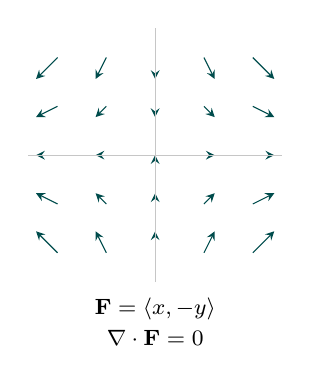
\begin{tikzpicture}[scale=0.62, every node/.style={font=\footnotesize}]
    \foreach \i in {-2,-1,0,1,2}{
        \foreach \j in {-2,-1,0,1,2}{
            \pgfmathsetmacro{\dx}{0.22*\i}
            \pgfmathsetmacro{\dy}{-0.22*\j}
            \draw[-stealth, teal!60!black] (\i,\j) -- ++(\dx,\dy);
        }
    }
    \draw[gray!45] (-2.6,0) -- (2.6,0);
    \draw[gray!45] (0,-2.6) -- (0,2.6);
    \node at (0,-3.15) {$\mathbf{F}=\langle x,-y\rangle$};
    \node at (0,-3.75) {$\nabla\cdot\mathbf{F}=0$};
\end{tikzpicture}
\hspace{0.4cm}
% div > 0 : F = (x, y)
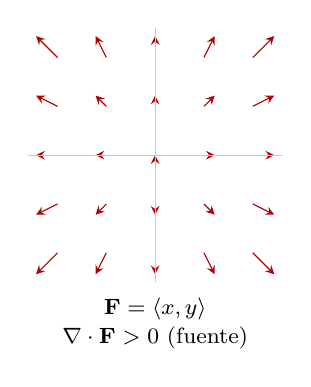
\begin{tikzpicture}[scale=0.62, every node/.style={font=\footnotesize}]
    \foreach \i in {-2,-1,0,1,2}{
        \foreach \j in {-2,-1,0,1,2}{
            \pgfmathsetmacro{\dx}{0.22*\i}
            \pgfmathsetmacro{\dy}{0.22*\j}
            \draw[-stealth, red!70!black] (\i,\j) -- ++(\dx,\dy);
        }
    }
    \draw[gray!45] (-2.6,0) -- (2.6,0);
    \draw[gray!45] (0,-2.6) -- (0,2.6);
    \node at (0,-3.15) {$\mathbf{F}=\langle x,y\rangle$};
    \node at (0,-3.75) {$\nabla\cdot\mathbf{F}>0$ (fuente)};
\end{tikzpicture}
\hspace{0.4cm}
% div < 0 : F = (-x, -y)
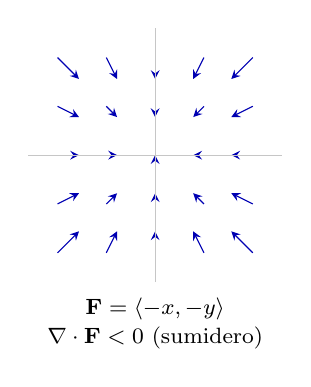
\begin{tikzpicture}[scale=0.62, every node/.style={font=\footnotesize}]
    \foreach \i in {-2,-1,0,1,2}{
        \foreach \j in {-2,-1,0,1,2}{
            \pgfmathsetmacro{\dx}{-0.22*\i}
            \pgfmathsetmacro{\dy}{-0.22*\j}
            \draw[-stealth, blue!70!black] (\i,\j) -- ++(\dx,\dy);
        }
    }
    \draw[gray!45] (-2.6,0) -- (2.6,0);
    \draw[gray!45] (0,-2.6) -- (0,2.6);
    \node at (0,-3.15) {$\mathbf{F}=\langle -x,-y\rangle$};
    \node at (0,-3.75) {$\nabla\cdot\mathbf{F}<0$ (sumidero)};
\end{tikzpicture}
\end{center}

En el campo central, el flujo que entra por el eje vertical se compensa con el que sale por el horizontal, de modo que la divergencia es cero pese a que el campo no es constante.

\subsection{Rotacional}

\begin{mydefinition}{Rotacional}
Sea $\mathbf{F} = \langle P, Q, R \rangle$ un campo vectorial diferenciable. Su rotacional es el campo vectorial:
\[
\operatorname{rot} \mathbf{F} = \nabla \times \mathbf{F}
= \left\langle
\frac{\partial R}{\partial y} - \frac{\partial Q}{\partial z},\;
\frac{\partial P}{\partial z} - \frac{\partial R}{\partial x},\;
\frac{\partial Q}{\partial x} - \frac{\partial P}{\partial y}
\right\rangle.
\]
\end{mydefinition}

El rotacional mide la tendencia del campo a inducir un giro local. Su dirección es el eje de rotación y su magnitud, la intensidad del giro. Para un campo plano $\mathbf{F} = \langle P, Q, 0 \rangle$ solo sobrevive la componente $z$:
\[
\nabla \times \mathbf{F} = \left( \frac{\partial Q}{\partial x} - \frac{\partial P}{\partial y} \right) \mathbf{k},
\]
cuyo signo distingue el sentido del giro: positiva para rotación en sentido antihorario y negativa para el horario. Un campo con rotacional nulo se llama irrotacional.

\textbf{Cálculo.} Para $\mathbf{F} = \langle xy,\; yz,\; zx \rangle$:
\[
\nabla \times \mathbf{F}
= \left\langle
\frac{\partial(zx)}{\partial y} - \frac{\partial(yz)}{\partial z},\;
\frac{\partial(xy)}{\partial z} - \frac{\partial(zx)}{\partial x},\;
\frac{\partial(yz)}{\partial x} - \frac{\partial(xy)}{\partial y}
\right\rangle
= \langle -y,\, -z,\, -x \rangle.
\]

Los tres campos planos siguientes ilustran los signos posibles de la componente $z$ del rotacional.

\begin{center}
\shorthandoff{>}
% rot = 0 : F = (y, x)
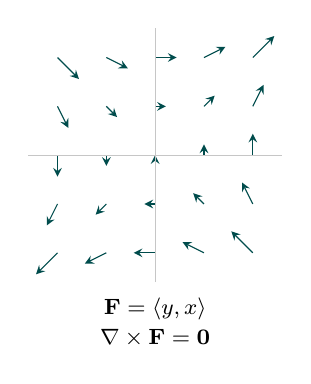
\begin{tikzpicture}[scale=0.62, every node/.style={font=\footnotesize}]
    \foreach \i in {-2,-1,0,1,2}{
        \foreach \j in {-2,-1,0,1,2}{
            \pgfmathsetmacro{\dx}{0.22*\j}
            \pgfmathsetmacro{\dy}{0.22*\i}
            \draw[-stealth, teal!60!black] (\i,\j) -- ++(\dx,\dy);
        }
    }
    \draw[gray!45] (-2.6,0) -- (2.6,0);
    \draw[gray!45] (0,-2.6) -- (0,2.6);
    \node at (0,-3.15) {$\mathbf{F}=\langle y,x\rangle$};
    \node at (0,-3.75) {$\nabla\times\mathbf{F}=\mathbf{0}$};
\end{tikzpicture}
\hspace{0.4cm}
% rot > 0 : F = (-y, x)
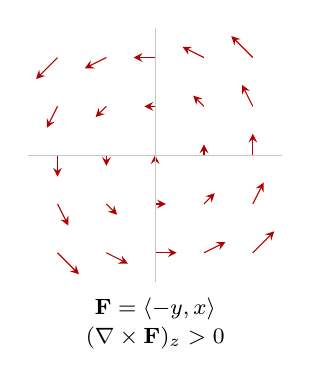
\begin{tikzpicture}[scale=0.62, every node/.style={font=\footnotesize}]
    \foreach \i in {-2,-1,0,1,2}{
        \foreach \j in {-2,-1,0,1,2}{
            \pgfmathsetmacro{\dx}{-0.22*\j}
            \pgfmathsetmacro{\dy}{0.22*\i}
            \draw[-stealth, red!70!black] (\i,\j) -- ++(\dx,\dy);
        }
    }
    \draw[gray!45] (-2.6,0) -- (2.6,0);
    \draw[gray!45] (0,-2.6) -- (0,2.6);
    \node at (0,-3.15) {$\mathbf{F}=\langle -y,x\rangle$};
    \node at (0,-3.75) {$(\nabla\times\mathbf{F})_z>0$};
\end{tikzpicture}
\hspace{0.4cm}
% rot < 0 : F = (y, -x)
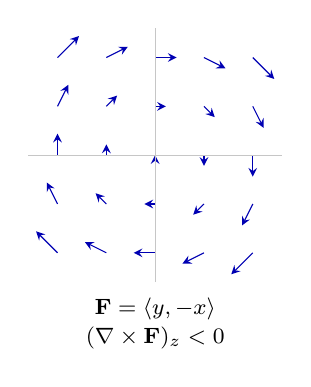
\begin{tikzpicture}[scale=0.62, every node/.style={font=\footnotesize}]
    \foreach \i in {-2,-1,0,1,2}{
        \foreach \j in {-2,-1,0,1,2}{
            \pgfmathsetmacro{\dx}{0.22*\j}
            \pgfmathsetmacro{\dy}{-0.22*\i}
            \draw[-stealth, blue!70!black] (\i,\j) -- ++(\dx,\dy);
        }
    }
    \draw[gray!45] (-2.6,0) -- (2.6,0);
    \draw[gray!45] (0,-2.6) -- (0,2.6);
    \node at (0,-3.15) {$\mathbf{F}=\langle y,-x\rangle$};
    \node at (0,-3.75) {$(\nabla\times\mathbf{F})_z<0$};
\end{tikzpicture}
\end{center}

El campo de la izquierda, aunque curva sus flechas, es el gradiente de $\varphi = xy$ y no produce giro neto: es irrotacional. Los otros dos giran en sentidos opuestos.

\subsection{Propiedades}

Las siguientes identidades relacionan el gradiente, la divergencia y el rotacional. En ellas $\varphi$ es un campo escalar y $\mathbf{F}$, $\mathbf{G}$ campos vectoriales, todos con las derivadas continuas necesarias.
\begin{align}
\nabla \cdot (\nabla \times \mathbf{F}) &= 0, \\
\nabla \times (\nabla \varphi) &= \mathbf{0}, \\
\nabla \cdot (\varphi\, \mathbf{F}) &= \varphi\, (\nabla \cdot \mathbf{F}) + \nabla \varphi \cdot \mathbf{F}, \\
\nabla \times (\varphi\, \mathbf{F}) &= \varphi\, (\nabla \times \mathbf{F}) + \nabla \varphi \times \mathbf{F}, \\
\nabla \cdot (\mathbf{F} \times \mathbf{G}) &= \mathbf{G} \cdot (\nabla \times \mathbf{F}) - \mathbf{F} \cdot (\nabla \times \mathbf{G}), \\
\nabla \times (\nabla \times \mathbf{F}) &= \nabla (\nabla \cdot \mathbf{F}) - \nabla^2 \mathbf{F}.
\end{align}

\subsection{Ejemplo de demostración clásica}

Para apreciar el trabajo que implica demostrar estas identidades por el método directo, se prueba la propiedad (5), $\nabla \cdot (\mathbf{F} \times \mathbf{G}) = \mathbf{G} \cdot (\nabla \times \mathbf{F}) - \mathbf{F} \cdot (\nabla \times \mathbf{G})$, desarrollando todas las componentes.

Con $\mathbf{F} = \langle F_1, F_2, F_3 \rangle$ y $\mathbf{G} = \langle G_1, G_2, G_3 \rangle$, las componentes del producto cruz son:
\[
\mathbf{F} \times \mathbf{G} = \langle F_2 G_3 - F_3 G_2,\; F_3 G_1 - F_1 G_3,\; F_1 G_2 - F_2 G_1 \rangle.
\]
Tomando la divergencia se derivan las tres componentes:
\[
\nabla \cdot (\mathbf{F} \times \mathbf{G})
= \frac{\partial}{\partial x}(F_2 G_3 - F_3 G_2)
+ \frac{\partial}{\partial y}(F_3 G_1 - F_1 G_3)
+ \frac{\partial}{\partial z}(F_1 G_2 - F_2 G_1).
\]
Aplicando la regla del producto a cada uno de los seis términos se obtienen doce sumandos:
\[
\begin{aligned}
\nabla \cdot (\mathbf{F} \times \mathbf{G}) =\;
& (\partial_x F_2)\,G_3 + F_2\,(\partial_x G_3) - (\partial_x F_3)\,G_2 - F_3\,(\partial_x G_2) \\
+\; & (\partial_y F_3)\,G_1 + F_3\,(\partial_y G_1) - (\partial_y F_1)\,G_3 - F_1\,(\partial_y G_3) \\
+\; & (\partial_z F_1)\,G_2 + F_1\,(\partial_z G_2) - (\partial_z F_2)\,G_1 - F_2\,(\partial_z G_1).
\end{aligned}
\]
Se reagrupan primero los sumandos en que la derivada recae sobre $\mathbf{F}$, factorizando las componentes de $\mathbf{G}$:
\[
G_1(\partial_y F_3 - \partial_z F_2) + G_2(\partial_z F_1 - \partial_x F_3) + G_3(\partial_x F_2 - \partial_y F_1)
= \mathbf{G} \cdot (\nabla \times \mathbf{F}).
\]
Luego los sumandos en que la derivada recae sobre $\mathbf{G}$, factorizando las componentes de $\mathbf{F}$:
\[
F_1(\partial_z G_2 - \partial_y G_3) + F_2(\partial_x G_3 - \partial_z G_1) + F_3(\partial_y G_1 - \partial_x G_2)
= -\,\mathbf{F} \cdot (\nabla \times \mathbf{G}).
\]
Sumando ambos grupos se llega a la identidad buscada:
\[
\nabla \cdot (\mathbf{F} \times \mathbf{G}) = \mathbf{G} \cdot (\nabla \times \mathbf{F}) - \mathbf{F} \cdot (\nabla \times \mathbf{G}). \qquad \square
\]
El procedimiento es correcto pero laborioso: exige escribir doce términos, controlar sus signos y reconocer las agrupaciones que reconstruyen cada rotacional. Para identidades con segundas derivadas, como (6), el volumen de términos crece aún más.

\subsection{Notación tensorial}

La notación tensorial, también llamada notación de índices, es una forma corta de escribir las operaciones con vectores. En lugar de escribir por separado las componentes $x$, $y$ y $z$, usamos letras como $i$, $j$ y $k$. Esto ayuda a hacer demostraciones más cortas y a detectar términos que se cancelan.

Usaremos las coordenadas usuales de $\mathbb{R}^3$:
\[
i,j,k,l,m \in \{1,2,3\},
\qquad
(x_1,x_2,x_3)=(x,y,z).
\]

\begin{mynote}{Reglas básicas para leer índices}
Un número no lleva índice; un vector se escribe $a_i$ y una matriz se escribe $A_{ij}$. Por ejemplo, $a_1$, $a_2$ y $a_3$ son las tres componentes de $\mathbf{a}$.

\emph{Regla de suma de Einstein.} Cuando un índice aparece dos veces en el mismo producto, se suman sus tres valores, aunque no aparezca el signo $\sum$. Por ejemplo,
\[
a_i b_i=\sum_{i=1}^{3}a_i b_i,
\qquad
A_{ij}b_j=\sum_{j=1}^{3}A_{ij}b_j.
\]
El índice que aparece una sola vez indica la componente que queda al final. Debe coincidir en ambos lados de la igualdad: $A_{ij}b_j=c_i$ representa tres ecuaciones, una por cada valor de $i$. En cambio, $a_i b_i=c$ da un solo número. El índice que se suma puede cambiarse de letra: $A_{ij}b_j=A_{ik}b_k$. No se debe repetir un mismo índice tres veces en un producto.

\emph{Derivadas.} Se escribe $\partial_i$ en lugar de $\dfrac{\partial}{\partial x_i}$. Si las derivadas segundas de $f$ son continuas, se puede cambiar el orden de derivación:
\[
\partial_i\partial_j f=\partial_j\partial_i f.
\]
\end{mynote}

\subsubsection*{Dos símbolos que simplifican cálculos}

La delta de Kronecker funciona como un selector: vale $1$ cuando los dos índices son iguales y vale $0$ cuando son distintos:
\[
\delta_{ij}=
\begin{cases}
1,& i=j,\\
0,& i\ne j.
\end{cases}
\]
Por eso permite reemplazar índices de forma inmediata:
\begin{align*}
\delta_{ij}a_j&=a_i, &
\delta_{ij}A_{jk}&=A_{ik}, &
\delta_{ii}&=3, &
\delta_{ij}\delta_{jk}&=\delta_{ik}.
\end{align*}
También es útil recordar que $\partial_i x_j=\delta_{ij}$ y $\partial_i x_i=3$.

El símbolo de Levi-Civita sirve para escribir el producto cruz. Su valor es
\[
\varepsilon_{ijk}=
\begin{cases}
+1,& (i,j,k)\text{ es una permutación par de }(1,2,3),\\
-1,& (i,j,k)\text{ es una permutación impar},\\
0,& \text{alguno de los índices coincide}.
\end{cases}
\]
En la práctica, lo importante es que al intercambiar dos índices cambia de signo. Si solo se mueven en ciclo, no cambia:
\[
\varepsilon_{ijk}=-\varepsilon_{jik}=-\varepsilon_{ikj},
\qquad
\varepsilon_{ijk}=\varepsilon_{jki}=\varepsilon_{kij}.
\]
Cuando aparecen dos símbolos $\varepsilon$, se pueden convertir en deltas. Las relaciones que más se usan son
\begin{align*}
\varepsilon_{ijk}\varepsilon_{ilm}
  &=\delta_{jl}\delta_{km}-\delta_{jm}\delta_{kl},\\
\varepsilon_{ijk}\varepsilon_{ijl}
  &=2\delta_{kl},
\qquad
\varepsilon_{ijk}\varepsilon_{ijk}=6.
\end{align*}
La primera de estas fórmulas es la más importante para demostrar identidades de productos cruzados.

\subsubsection*{Una cancelación muy útil}

Si una expresión no cambia al intercambiar $i$ y $j$, se dice que es simétrica; si cambia de signo, se dice que es antisimétrica. Al multiplicar y sumar una de cada tipo, el resultado es cero:
\[
S_{ij}=S_{ji},\quad A_{ij}=-A_{ji}
\qquad\Longrightarrow\qquad
S_{ij}A_{ij}=0.
\]
La razón es sencilla: al cambiar $i$ por $j$, la suma es la misma, pero también adquiere un signo menos; por tanto, solo puede valer cero. Esta idea explica por qué $\nabla\cdot(\nabla\times\mathbf{F})=0$ y $\nabla\times(\nabla\varphi)=\mathbf{0}$: las derivadas dobles se pueden intercambiar, pero $\varepsilon_{ijk}$ cambia de signo.

\subsubsection*{Fórmulas para usar en demostraciones}

Para vectores $\mathbf{a}$ y $\mathbf{b}$, un campo escalar $f$ y un campo vectorial $\mathbf{F}$, las fórmulas básicas son
\begin{align*}
\mathbf{a}\cdot\mathbf{b}&=a_i b_i,
&
(\mathbf{a}\times\mathbf{b})_i&=\varepsilon_{ijk}a_jb_k,\\
(\nabla f)_i&=\partial_i f,
&
\nabla\cdot\mathbf{F}&=\partial_iF_i,
&
(\nabla\times\mathbf{F})_i&=\varepsilon_{ijk}\partial_jF_k,\\
\nabla^2f&=\partial_i\partial_i f,
&
(\nabla^2\mathbf{F})_i&=\partial_j\partial_jF_i.
\end{align*}
La regla del producto se usa igual que siempre:
\[
\partial_i(fg)=(\partial_i f)g+f(\partial_i g),
\qquad
\partial_i(F_jG_k)=(\partial_iF_j)G_k+F_j(\partial_iG_k).
\]
Por último, de las fórmulas con $\varepsilon$ se obtienen estas identidades conocidas:
\begin{align*}
\mathbf{a}\times(\mathbf{b}\times\mathbf{c})
  &=\mathbf{b}\,(\mathbf{a}\cdot\mathbf{c})-\mathbf{c}\,(\mathbf{a}\cdot\mathbf{b}),\\
(\mathbf{a}\times\mathbf{b})\cdot(\mathbf{c}\times\mathbf{d})
  &=(\mathbf{a}\cdot\mathbf{c})(\mathbf{b}\cdot\mathbf{d})
    -(\mathbf{a}\cdot\mathbf{d})(\mathbf{b}\cdot\mathbf{c}),\\
\|\mathbf{a}\times\mathbf{b}\|^2
  &=\|\mathbf{a}\|^2\|\mathbf{b}\|^2-(\mathbf{a}\cdot\mathbf{b})^2.
\end{align*}
Para intercambiar el orden de dos derivadas parciales, hay que comprobar que las derivadas segundas existen y son continuas.

\subsection{Divergencia y rotacional en notación tensorial}

Con estas convenciones, los operadores diferenciales se escriben de forma compacta. Para un campo escalar $\varphi$ y un campo vectorial $\mathbf{F}$ de componentes $F_i$:
\[
(\nabla \varphi)_i = \partial_i \varphi,
\qquad
\nabla \cdot \mathbf{F} = \partial_i F_i,
\qquad
(\nabla \times \mathbf{F})_i = \varepsilon_{ijk}\, \partial_j F_k.
\]
El producto punto y el producto cruz siguen el mismo patrón:
\[
\mathbf{a} \cdot \mathbf{b} = a_i b_i,
\qquad
(\mathbf{a} \times \mathbf{b})_i = \varepsilon_{ijk}\, a_j b_k.
\]
La divergencia contrae en un solo índice la derivada con la componente; el rotacional usa $\varepsilon_{ijk}$ para producir, en la componente $i$, la combinación antisimétrica de las derivadas cruzadas.

\subsection{Ejemplo de demostración con notación tensorial}

Se demuestra la misma propiedad (5) con esta notación, para contrastar con el desarrollo clásico. Partiendo de $(\mathbf{F} \times \mathbf{G})_i = \varepsilon_{ijk}\, F_j G_k$:
\[
\nabla \cdot (\mathbf{F} \times \mathbf{G})
= \partial_i \bigl( \varepsilon_{ijk}\, F_j G_k \bigr)
= \varepsilon_{ijk}\, (\partial_i F_j)\, G_k + \varepsilon_{ijk}\, F_j\, (\partial_i G_k).
\]
En el primer término, la antisimetría $\varepsilon_{ijk} = \varepsilon_{kij}$ permite escribir $\varepsilon_{ijk}\, \partial_i F_j = (\nabla \times \mathbf{F})_k$, de modo que el término es $G_k (\nabla \times \mathbf{F})_k = \mathbf{G} \cdot (\nabla \times \mathbf{F})$. En el segundo, $\varepsilon_{ijk} = -\varepsilon_{jik}$ da $\varepsilon_{ijk}\, \partial_i G_k = -(\nabla \times \mathbf{G})_j$, y el término es $-F_j (\nabla \times \mathbf{G})_j = -\mathbf{F} \cdot (\nabla \times \mathbf{G})$. Por tanto:
\[
\nabla \cdot (\mathbf{F} \times \mathbf{G}) = \mathbf{G} \cdot (\nabla \times \mathbf{F}) - \mathbf{F} \cdot (\nabla \times \mathbf{G}). \qquad \square
\]
El mismo resultado que antes ocupó doce términos se obtiene ahora en tres pasos. Como segunda muestra del poder de la notación, las identidades (1) y (2) se reducen a una línea cada una:
\[
\nabla \cdot (\nabla \times \mathbf{F}) = \varepsilon_{ijk}\, \partial_i \partial_j F_k = 0,
\qquad
(\nabla \times \nabla \varphi)_i = \varepsilon_{ijk}\, \partial_j \partial_k \varphi = 0,
\]
pues en ambos casos $\varepsilon_{ijk}$ es antisimétrico en dos índices sobre los que la doble derivada parcial es simétrica, y la contracción de un objeto antisimétrico con uno simétrico es nula.

\subsection{Ejercicios}

Los ejercicios están ordenados de menor a mayor dificultad. Intenta resolverlos antes de consultar las secciones anteriores.
\begin{enumerate}
    \item Sea $\mathbf{F}(x,y)=\langle 2x-y,\,x+y\rangle$.
\begin{enumerate}
    \item Calcule $\mathbf{F}(1,0)$ y $\mathbf{F}(-1,2)$.
    \item Calcule la magnitud de $\mathbf{F}(1,0)$.
    \item Indique hacia dónde apunta el vector $\mathbf{F}(1,0)$ en el plano.
\end{enumerate}

    \item Considere el campo vectorial
\[
\mathbf{F}(x,y,z)=\left\langle \frac{x}{x^2+y^2},\,\frac{y}{x^2+y^2},\,z\right\rangle.
\]
Determine el dominio de $\mathbf{F}$. Explique qué puntos no pertenecen al dominio.

    \item El campo $\mathbf{V}(x,y)=\langle -y,\,x\rangle$ representa un movimiento de giro alrededor del origen.
\begin{enumerate}
    \item Calcule $\mathbf{V}(1,0)$, $\mathbf{V}(0,1)$, $\mathbf{V}(-1,0)$ y $\mathbf{V}(0,-1)$.
    \item Dibuje estos cuatro vectores en sus respectivos puntos.
    \item Con base en el dibujo, indique si el giro es horario o antihorario.
\end{enumerate}

    \item Sea $f(x,y,z)=x^2y+3yz^2-x$.
\begin{enumerate}
    \item Calcule el gradiente $\nabla f$.
    \item Evalúe $\nabla f$ en el punto $(1,1,0)$.
    \item Escriba la derivada direccional de $f$ en $(1,1,0)$ en la dirección del vector $\mathbf{v}=\langle 1,2,2\rangle$.
\end{enumerate}

    \item Sea $f(x,y)=x^2-2xy+3y^2$.
\begin{enumerate}
    \item Calcule el campo $\mathbf{F}=\nabla f$.
    \item Calcule $\mathbf{F}(1,-1)$.
    \item Verifique que el vector obtenido es perpendicular a la curva de nivel de $f$ que pasa por $(1,-1)$.
\end{enumerate}

    \item Calcule la divergencia de cada campo e indique si, en el punto señalado, se comporta como fuente, sumidero o ninguno de los dos.
\begin{enumerate}
    \item $\mathbf{F}(x,y)=\langle x,\,y\rangle$ en $(0,0)$.
    \item $\mathbf{G}(x,y)=\langle -2x,\,-2y\rangle$ en $(1,-1)$.
    \item $\mathbf{H}(x,y)=\langle y,\,-x\rangle$ en $(2,0)$.
\end{enumerate}

    \item Sea $\mathbf{F}(x,y,z)=\langle x^2z,\,-2xyz,\,xy^2\rangle$.
\begin{enumerate}
    \item Calcule $\nabla\cdot\mathbf{F}$.
    \item Decida si el campo es solenoidal.
    \item Explique qué significa su respuesta en términos de flujo que entra y sale de una región pequeña.
\end{enumerate}

    \item Para cada campo plano, calcule la componente $z$ del rotacional e indique el sentido de giro cuando sea distinto de cero.
\begin{enumerate}
    \item $\mathbf{F}(x,y)=\langle -2y,\,2x\rangle$.
    \item $\mathbf{G}(x,y)=\langle 3x+y,\,x-2y\rangle$.
    \item $\mathbf{H}(x,y)=\langle 2xy,\,x^2-y^2\rangle$.
\end{enumerate}

    \item Sea
\[
\mathbf{F}(x,y,z)=\langle yz,\,xz,\,xy\rangle.
\]
Calcule $\nabla\cdot\mathbf{F}$ y $\nabla\times\mathbf{F}$. A partir de los resultados, determine si el campo es solenoidal, irrotacional, ambos o ninguno.

    \item Sean $f(x,y,z)=x^2y$ y $\mathbf{F}(x,y,z)=\langle x,\,y,\,z\rangle$.
\begin{enumerate}
    \item Calcule directamente $\nabla\cdot(f\mathbf{F})$.
    \item Calcule $f(\nabla\cdot\mathbf{F})+\nabla f\cdot\mathbf{F}$.
    \item Compruebe que ambos resultados son iguales.
\end{enumerate}

    \item Determine cuáles de los siguientes campos planos pueden ser conservativos en todo $\mathbb{R}^2$. Justifique comparando las derivadas cruzadas $\partial P/\partial y$ y $\partial Q/\partial x$.
\begin{enumerate}
    \item $\mathbf{F}(x,y)=\langle 2x+y,\,x+4y\rangle$.
    \item $\mathbf{G}(x,y)=\langle y^2,\,2xy+1\rangle$.
    \item $\mathbf{H}(x,y)=\langle -y,\,x\rangle$.
\end{enumerate}

    \item Encuentre una función potencial $\varphi$ para el campo
\[
\mathbf{F}(x,y)=\langle 3x^2+2y,\,2x-4y\rangle.
\]
Después, verifique que $\nabla\varphi=\mathbf{F}$ y calcule el cambio de potencial entre los puntos $A=(0,0)$ y $B=(1,2)$.

    \item Considere el campo radial
\[
\mathbf{F}(x,y,z)=\langle x,\,y,\,z\rangle.
\]
\begin{enumerate}
    \item Calcule su divergencia y su rotacional.
    \item Encuentre una función potencial para $\mathbf{F}$.
    \item Explique por qué las flechas del campo apuntan hacia afuera del origen.
\end{enumerate}

    \item Sea $\mathbf{F}(x,y,z)=\langle xz,\,yz,\,xy\rangle$.
\begin{enumerate}
    \item Calcule $\nabla\times\mathbf{F}$.
    \item Calcule $\nabla\cdot(\nabla\times\mathbf{F})$.
    \item Calcule $\nabla\cdot\mathbf{F}$ y después $\nabla(\nabla\cdot\mathbf{F})$.
    \item Calcule $\nabla^2\mathbf{F}$ y compruebe la identidad
    \[
    \nabla\times(\nabla\times\mathbf{F})
    =\nabla(\nabla\cdot\mathbf{F})-\nabla^2\mathbf{F}.
    \]
\end{enumerate}

    \item Use notación de índices para demostrar que la divergencia de un rotacional es cero. Siga estos pasos para un campo $\mathbf{F}$ cuyas derivadas segundas sean continuas:
\begin{enumerate}
    \item Escriba $\nabla\cdot(\nabla\times\mathbf{F})$ como $\varepsilon_{ijk}\,\partial_i\partial_jF_k$.
    \item Explique qué ocurre con $\partial_i\partial_jF_k$ al intercambiar $i$ y $j$.
    \item Explique qué ocurre con $\varepsilon_{ijk}$ al intercambiar $i$ y $j$.
    \item Concluya que $\nabla\cdot(\nabla\times\mathbf{F})=0$.
\end{enumerate}

\end{enumerate}

